% !TeX root = repressed-anger.tex

\section{Classification Techniques}
\label{sec:algorithms}

The aim of this section has two purposes. The first one, is to make an introduction of the basic concepts of classification, which is essential for the detection of repressed anger as the solution proposed has been defined as a classification problem. The second one, is to explain how the algorithms used in this study work.

\subsection{Fundamentals of Classification}

According to \cite{voznika2007data}, classification can be defined as the task of predicting an outcome from a given input. This outcome is produced by the process of mapping a group of characteristics present in the input to a certain category. In other words, it consists in assigning objects (the input) to one of several predefined classes (the outcome) \cite{pang2006introduction}. Examples of classification can be found in everyday life, such as e-mail spam detection, news classifiers, \acrfull{ocr}, animal kingdom classification (see Figure \ref{fig:animal_classification}), among many others.

\begin{figure}[!htp]
  \center
  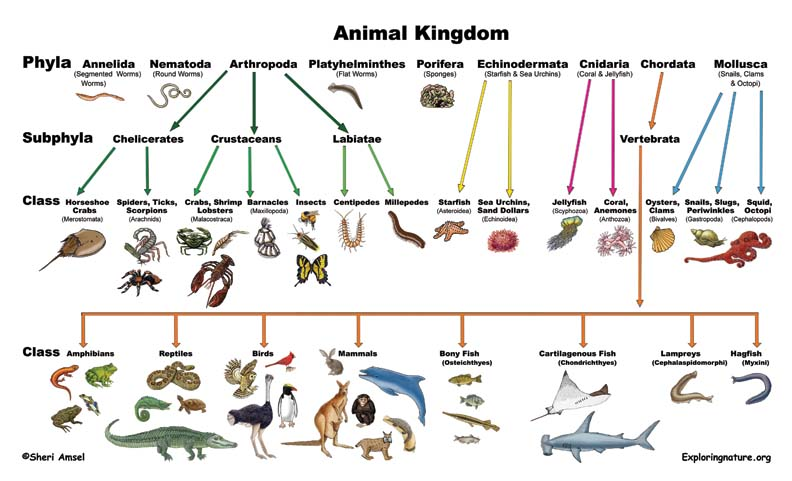
\includegraphics[width=0.85\textwidth]{figures/animal_classification}
  \caption{Classification of animals. The image is extracted from Exploring Nature.}
  \label{fig:animal_classification}
\end{figure}

\FloatBarrier

The input data for a classification task is composed by a collection of records, the dataset. In the same time, each record, also known as an instance, is composed by a set attributes. From all these attributes there is one considered special, which is called the target attribute or the class label. Regular attributes can be both discrete or continuous values. For the values signed for the class label, however, they must be discrete. This characteristic is what distinguishes classification form regression. Table \ref{tab:clasiffication_table} shows a sample dataset for animal classification into the following categories: amphibian, bird, fish or mammal.

\begin{table}[!htp]
\centering
\begin{tabular}{ |c|c|c|c|c|c|c|c| }
\hline
Common Name & Hair & Feathers & Eggs & Milk & Aquatic & Legs & Class Label \\ \hline
antelope & Yes & No & No & No & No & 4 & mammal \\ \hline
catfish & No & No & Yes & No & Yes & 0 & fish \\ \hline
dolphin & No & No & No & Yes & Yes & 0 & mammal \\ \hline
dove & No & Yes & Yes & No & No & 2 & bird \\ \hline
duck & No & Yes & Yes & No & Yes & 2 & bird \\ \hline
elephant & Yes & Yes & No & Yes & No & 4 & mammal \\ \hline
flamingo & Yes & Yes & Yes & No & No & 2 & bird \\ \hline
frog & No & No & Yes & No & Yes & 4 & amphibian \\ \hline
fruit bat & Yes & No & No & Yes & No & 2 & mammal \\ \hline
gull & No & Yes & Yes & No & Yes & 2 & bird \\ \hline
herring & No & No & Yes & No & Yes & 0 & fish \\ \hline
kiwi & No & No & Yes & No & No & 2 & bird \\ \hline
lark & No & Yes & Yes & No & No & 2 & bird \\ \hline
lynx & Yes & No & No & Yes & No & 4 & mammal \\ \hline
mole & Yes & No & No & Yes & No & 4 & mammal \\ \hline
mongoose & Yes & No & No & Yes & No & 4 & mammal \\ \hline
newt & No & No & Yes & No & Yes & 4 & amphibian \\
\hline
\end{tabular}
\caption{Animal kingdom dataset.}
\label{tab:clasiffication_table}
\end{table}

Tan Pang-Ning et al. propose a more mathematical definition of classification stating that it is the process of learning a target function $f$, also known as classification model, that maps each attribute set $x$ to one of the predefined class labels $y$.

\begin{figure}[!htp]
  \center
  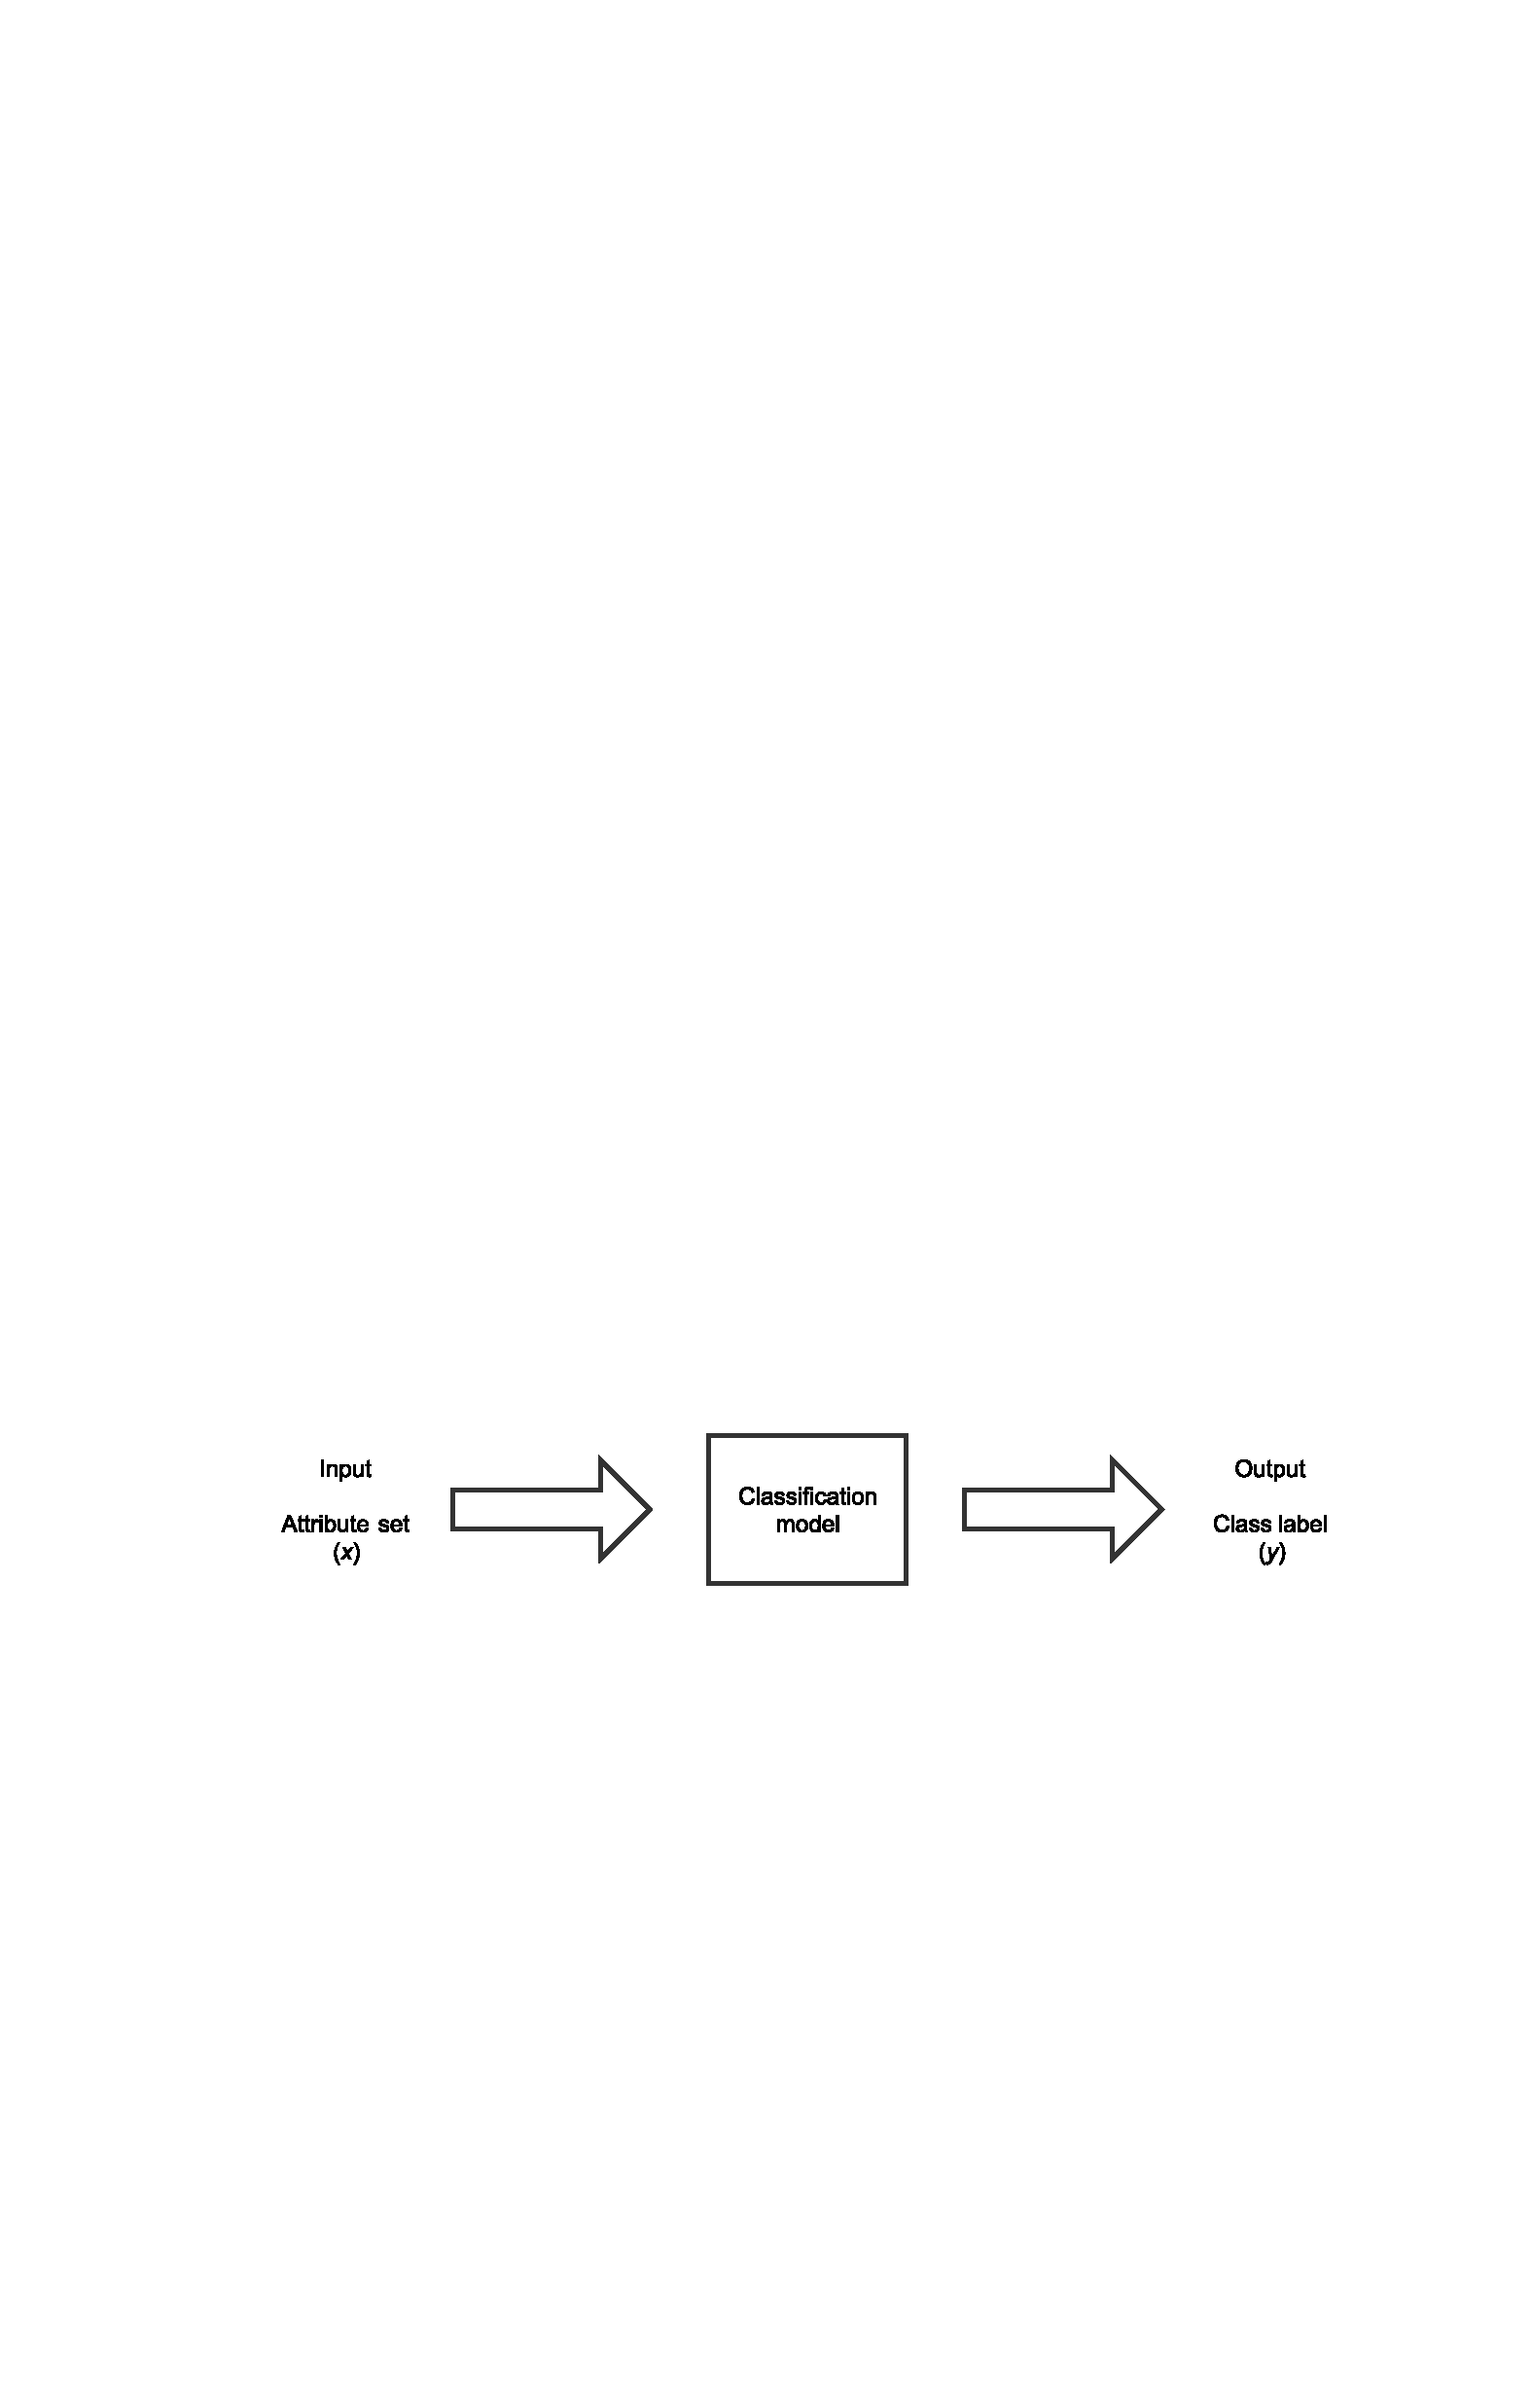
\includegraphics[width=\textwidth]{figures/classification}
  \caption{Classification as a task of mapping a set attributes $x$ into its fitting class label $y$.}
  \label{fig:classification_task}
\end{figure}

A classification model is useful for the following purposes \cite{pang2006introduction}:

\begin{itemize}
\item \textbf{Descriptive Modeling:} Since a classification model presents the main features of the data, it can serve as an explanatory tool to distinguish between instances of different categories \cite{madigan2002descriptive}.

\item \textbf{Predictive Modeling:} A classification model can also be used to predict the class label of an unknown new instance. As shown in Figure \ref{fig:classification_task}, a classification model can be represented as a black box that automatically assigns a class label to an instance by providing its attribute set.
\end{itemize}

It is important to remark that classification techniques perform their best when used for predicting or describing datasets which its class label is binary or nominal, Since they no consider properties such ordinality or the implicit order among the categories, they become ineffective with ordinal class labels \cite{frank2001simple}.

\subsection{General classification problem solving}
\label{general_classificartion_problem_solving}

For general classification problems solving, popular techniques consists on a process that starts with building classification models from a sample dataset \cite{witten2005data}. Each technique depends on a learning algorithm witch is in charge of generating the classification model. A good model should define the relationship between the input attribute set and its belonging category that suits the best. Therefore, the model should be valid for both, the sample data used to generate the model and also for new unknown instances. Among popular classification techniques, \acrfull{svm}, \acrfullpl{nn}, Naive Bayes or \acrfullpl{dt} can be found \cite{garje2016sentiment}.

\begin{figure}[!htp]
  \center
  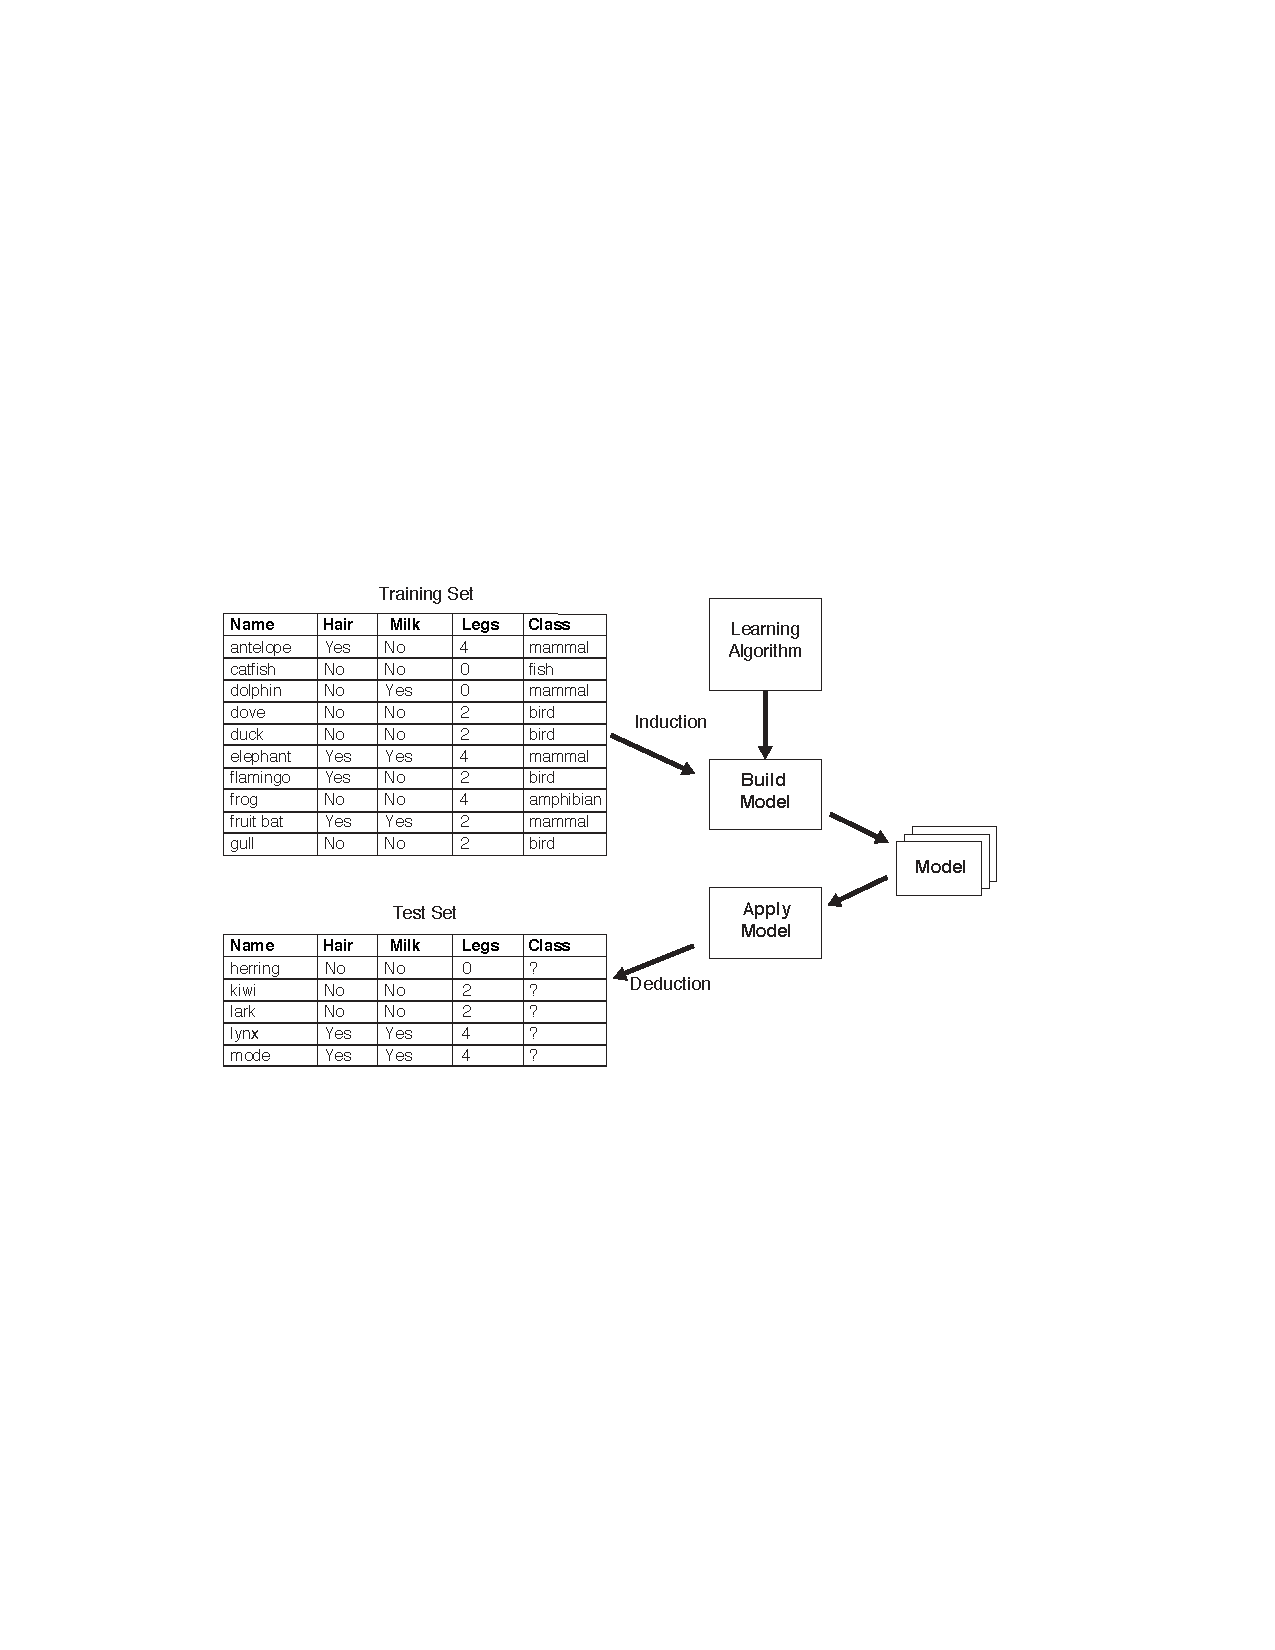
\includegraphics[width=0.85\textwidth]{figures/classification_problem_solving}
  \caption{General approach for classification model building and new instance category prediction.}
  \label{fig:classification_problem}
\end{figure}

As shown in the Figure \ref{fig:classification_problem}, to solve a classification problem a sample dataset must be provided as a training set. This sample is used to build the classification model according to the learning algorithm. After the model is built, it is applied to unlabeled dataset, also called the test set, to predict the categories of each instances of the records. To measure how good the model is, there is only need to count the number of instances have been correctly and incorrectly classified from the test set. Usually, to represent system's performance values, a confusion matrix is used \cite{hamilton2000confusion}. 


\begin{table}[!htp]
\centering
\begin{tabular}{ |c|c|c|c| }
\hline
\multicolumn{2}{|c|}{} & \multicolumn{2}{c|}{Predicted Class} \\
\hhline{~~--}
\multicolumn{2}{|c|}{} & $Class = Yes$ & $Class = No$ \\ \hline
\multirow{2}{*}{Actual Class} & $Class = Yes$ & a & b \\
\hhline{~---}
& $Class = No$ & c & d \\
\hline
\end{tabular}
\caption{Confusion matrix of a binary classification.}
\label{tab:confusion_matrix}
\end{table}

As a example, Table \ref{tab:confusion_matrix} represents the confusion matrix of a binary classification problem, in which the possible classes that can be assigned to a given instance are \textit{Yes} or \textit{No}. The values presented in this confusion matrix represents the counts of instances correctly and incorrectly classified as a means of evaluation of the model performance, being the diagonal of the table the instances classified correctly, the true positives (\acrshort{tp}) and negatives (\acrshort{tn}). The rest of the table corresponds to the number of instances that have been classified incorrectly, the false positives (\acrshort{fp}) and false negatives (\acrshort{fn}). The definition of a cell is done by the value of the column and the row in which is positioned, read as the number instances of \textit{X} classified as \textit{Y}, where \textit{X} and \textit{Y} are the determined value of the row and column respectively. For instance, the cell $a$ is interpreted as the counts of Yes that have been classified as \textit{Yes}, the TP.

Although the confusion matrix gives all the relevant information to determine how well the system has performed, sometimes is convenient to provide this information into a single value that summarizes the content of all the table. To do so, multiple performance metrics have been defined and one of those is the accuracy defined as:

\[Overall\ accuracy=\frac{TP+TN}{TP+FP+FN+TN}\]

Accuracy represents the percentage of correctly classified instances. However, using only accuracy may not be enough, as for example, when the dataset is imbalanced or it has a majority of elements for a determined class. For instance, on a naive classifier that always determined an instance as the element with the maximum number of appearances in the dataset, the accuracy of classifier results in a high value, although, the model does not have a real predictive capacity. This phenomena is considered the accuracy paradox \cite{accuracyParadox} and thus, to avoid the scoring a misleading measurement, it is recommendable to combine its usage with other performance metrics such as precision and recall.

By talking the definition of precision from information retrieval context, it would answer to the question \textit{how many classified items are relevant for the current query?} and thus, the precision is defined as:

\[Precision=\frac{TP}{TP+FP}\]

In the same context recall, in the other hand, answers to the question \textit{how many relevant items are classified properly?} and such, defined as:

\[Recall=\frac{TP}{TP+FN}\]

Finally, a combination of both measures, precision and recall, as a weighted average is called F-Measure or F1-Score. It allows to have a single performance metric to evaluate the classifier. Although, multiple definitions of the metric that give more relevance to the recall over the precision or vice versa exist, the general definition can be specified by the following equation:

\[F_1=2 \times \frac{precision \times recall}{precision+recall}\]

\iffalse

\subsection{Support Vector Machine}

There are four main advantages: Firstly it has a regularisation parameter, which makes the user think about avoiding over-fitting. Secondly it uses the kernel trick, so you can build in expert knowledge about the problem via engineering the kernel. Thirdly an SVM is defined by a convex optimisation problem (no local minima) for which there are efficient methods (e.g. SMO). Lastly, it is an approximation to a bound on the test error rate, and there is a substantial body of theory behind it which suggests it should be a good idea.
The disadvantages are that the theory only really covers the determination of the parameters for a given value of the regularisation and kernel parameters and choice of kernel. In a way the SVM moves the problem of over-fitting from optimising the parameters to model selection. Sadly kernel models can be quite sensitive to over-fitting the model selection criterion \cite{cawley2010over}

--------------------

SVMs are a new promising non-linear, non-parametric classification tech- nique, which already showed good results in the medical diagnostics, optical character recognition, elec- tric load forecasting and other fields.

Suitable for binary classification tasks.

The advantages of the SVM technique can be summarised as follows \cite{auria2008support}:

\begin{enumerate}
\item By introducing the kernel, SVMs gain flexibility in the choice of the form of the threshold separating solvent from insolvent companies, which needs not be linear and even needs not have the same func- tional form for all data, since its function is non-parametric and operates locally. As a consequence they can work with financial ratios, which show a non-monotone relation to the score and to the probability of default, or which are non-linearly dependent, and this without needing any specific work on each non-monotone variable.
\item Since the kernel implicitly contains a non-linear transformation, no assumptions about the functional form of the transformation, which makes data linearly separable, is necessary. The transformation oc- curs implicitly on a robust theoretical basis and human expertise judgement beforehand is not needed.
\item SVMs provide a good out-of-sample generalization, if the parameters C and r (in the case of a Gaussian kernel) are appropriately chosen. This means that, by choosing an appropriate generalization grade, SVMs can be robust, even when the training sample has some bias
\item SVMs deliver a unique solution, since the optimality problem is convex. This is an advantage compared to Neural Networks, which have multiple solutions associated with local minima and for this reason may not be robust over different samples.
\item With the choice of an appropriate kernel, such as the Gaussian kernel, one can put more stress on the similarity between companies, because the more similar the financial structure of two companies is, the higher is the value of the kernel. Thus when classifying a new company, the values of its financial ratios are compared with the ones of the support vectors of the training sample which are more similar to this new company. This company is then classified according to with which group it has the greatest similarity.
\end{enumerate}

--------------------------

Furthermore, $K(\bm{x}i, \bm{x}j ) \equiv \phi(\bm{x}_i)^T \phi(\bm{x}_j)$ is called the kernel function.

four basic kernels \cite{hsu2003practical}:

\begin{itemize}
\item \textbf{Linear:} $K(\bm{x}_i,\bm{x}_j) = \bm{x}^T_i \bm{x}_j$.
\item \textbf{Polynomial:} $K(\bm{x}_i,\bm{x}_j) = (\gamma \bm{x}^T_i \bm{x}_j + r)^d, \gamma > 0$.
\item \textbf{Radial Basis Function (RBF):} $K(\bm{x}_i,\bm{x}_j) = \exp(−\gamma \lVert \bm{x}_i − \bm{x}_j \rVert ^2),\gamma > 0$.
\item \textbf{Sigmoid:} $K(\bm{x}_i,\bm{x}_j) = \tanh(\gamma \bm{x}^T_i\bm{x}_j + r)$.
\end{itemize}

Here, $\gamma$, $r$, and $d$ are kernel parameters.

--------------------------

Support vector machines (SVM) were originally designed for binary classification \cite{hsu2002comparison}.

solving multi-class SVM in one step: “all-together” methods: [25], [27] and [7]. We then compare their performance with three methods based on binary classifications: “one-against-all,” “one-against-one,” and DAGSVM [23]. Our experiments indicate that the “one-against-one” and DAG methods are more suitable for practical use than the other methods. 

--------------------------

asdasdasd \cite{berwick2003idiot}

\begin{figure}[!htp]
  \center
  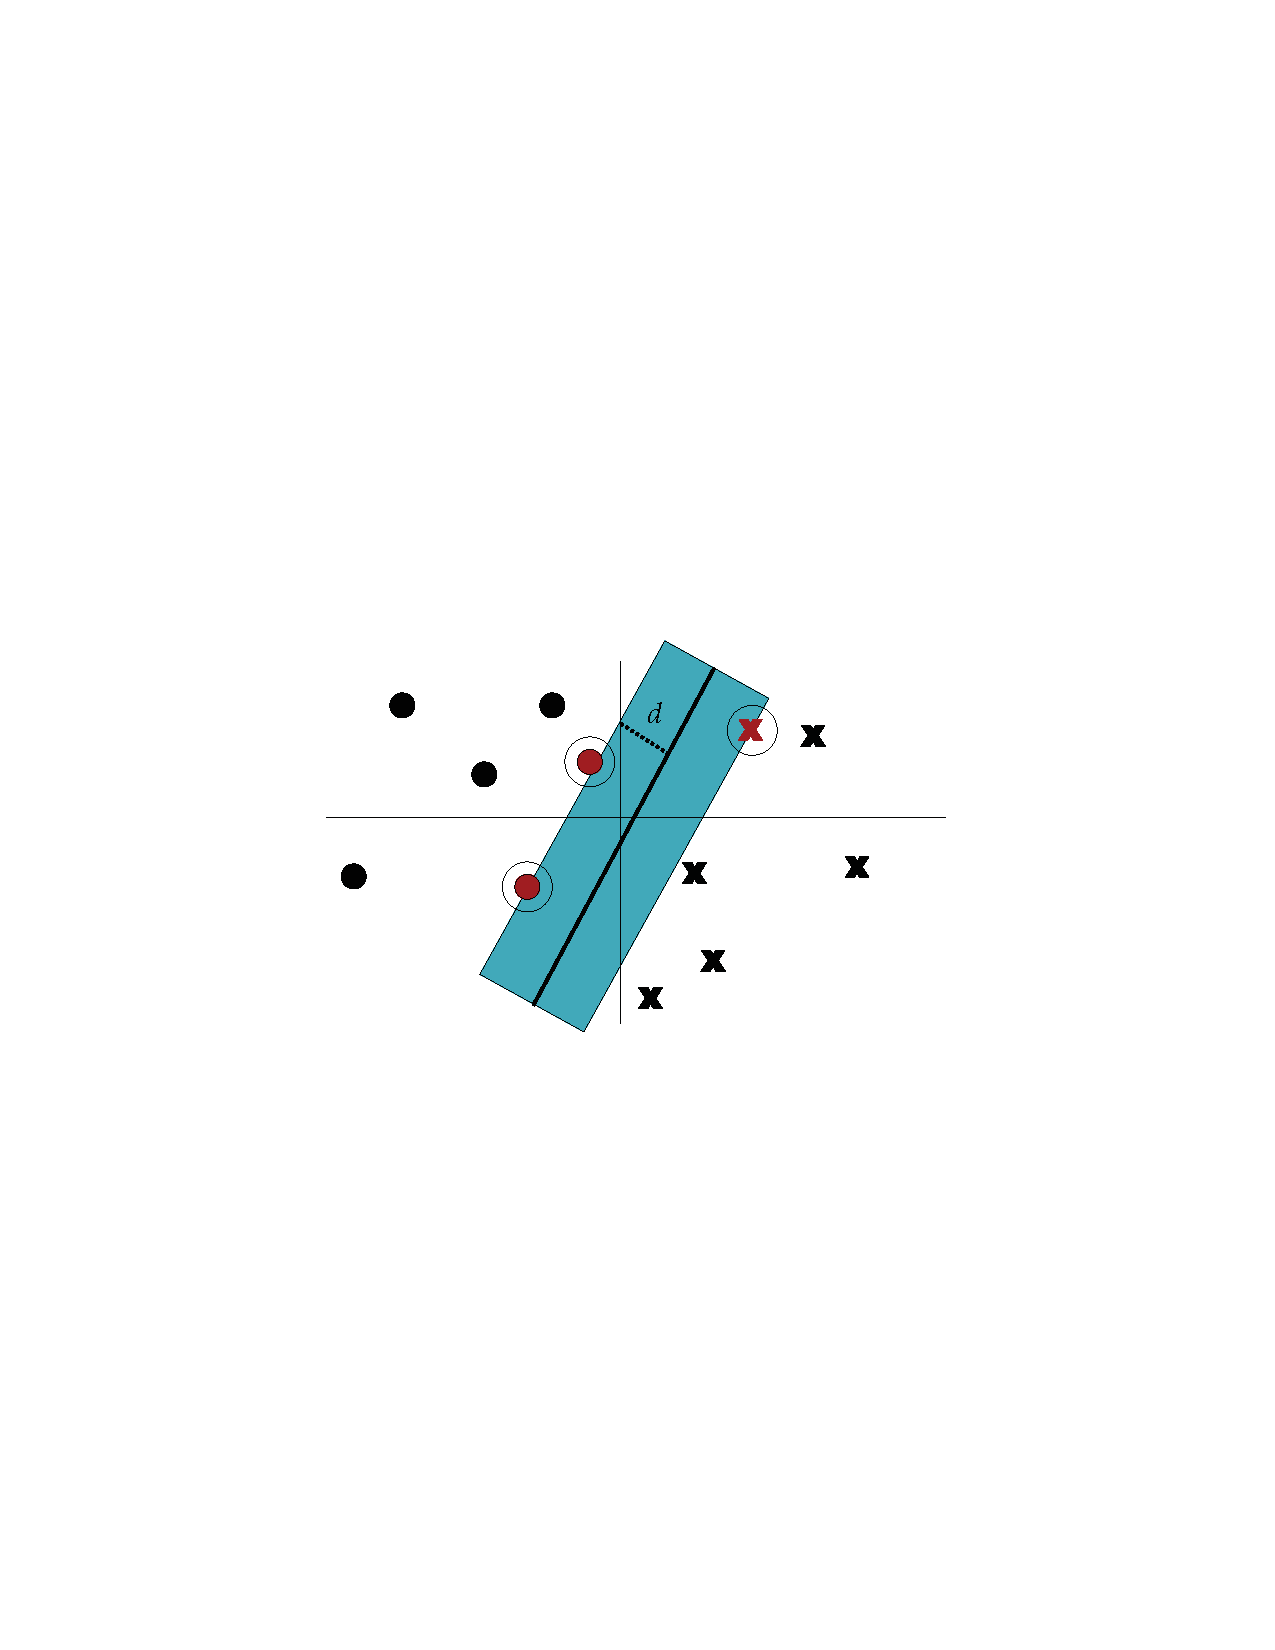
\includegraphics[width=0.6\textwidth]{figures/hyperplane}
  \caption{hyperplane}
  \label{fig:hyperplane}
\end{figure}

\subsection{K-Nearest Neighbor}

\subsection{Neural Networks}

\subsection{Ensemble Learning}
\label{subsec:ensemble_learning]}

\cite{ensemble2009Polikar}

\fi

\subsection{Deep Learning: Convolutional Neural Network}
\label{subsec:deep_learning}

In this section we will explain the fundamental of the algorithm on which our solution is basen on, \acrlong{cnn}, a technology that was designed thinking mainly on computer vision tasks, but has proven to also for well on \acrshort{nlp} \cite{zhang2015sensitivity}, \cite{kim2014convolutional}. To understand how \acrshort{cnn} work, first we need to understand what a convolution is.

\section{Convolution}

A convolution could be defined as an integral that denotes the amount of overlap that the function $g$ shifts over another function $f$ (see figure \ref{fig:representation_convolution}).

Mathematically, a convolution is the product of two functions $f$ and $g$. Depending on the values of the overlap are finite or not, the convolution (single dimension) could be defined as \cite{convolution}: 

\begin{figure}[!htp]
  \center
  \[[f \ast g](t)=\int_{0}^{t} f(\tau)g(t-\tau)d\tau\]
  \caption{Convolution for a finite range of $t \in [0, \infty]$}
  \label{fig:convolution_finite_range}
\end{figure}

or as:

\begin{figure}[!htp]
  \center
  \[f \ast g \equiv \int_{-\infty}^{\infty} f(\tau)g(t-\tau)d\tau\]\[=\int_{-\infty}^{\infty} g(\tau)f(t-\tau)d\tau\]
  \caption{Convolution for a infinite range of $t \in (-\infty, \infty)$}
  \label{fig:convolution_infinite_range}
\end{figure}

\begin{figure}[!htp]
  \center
  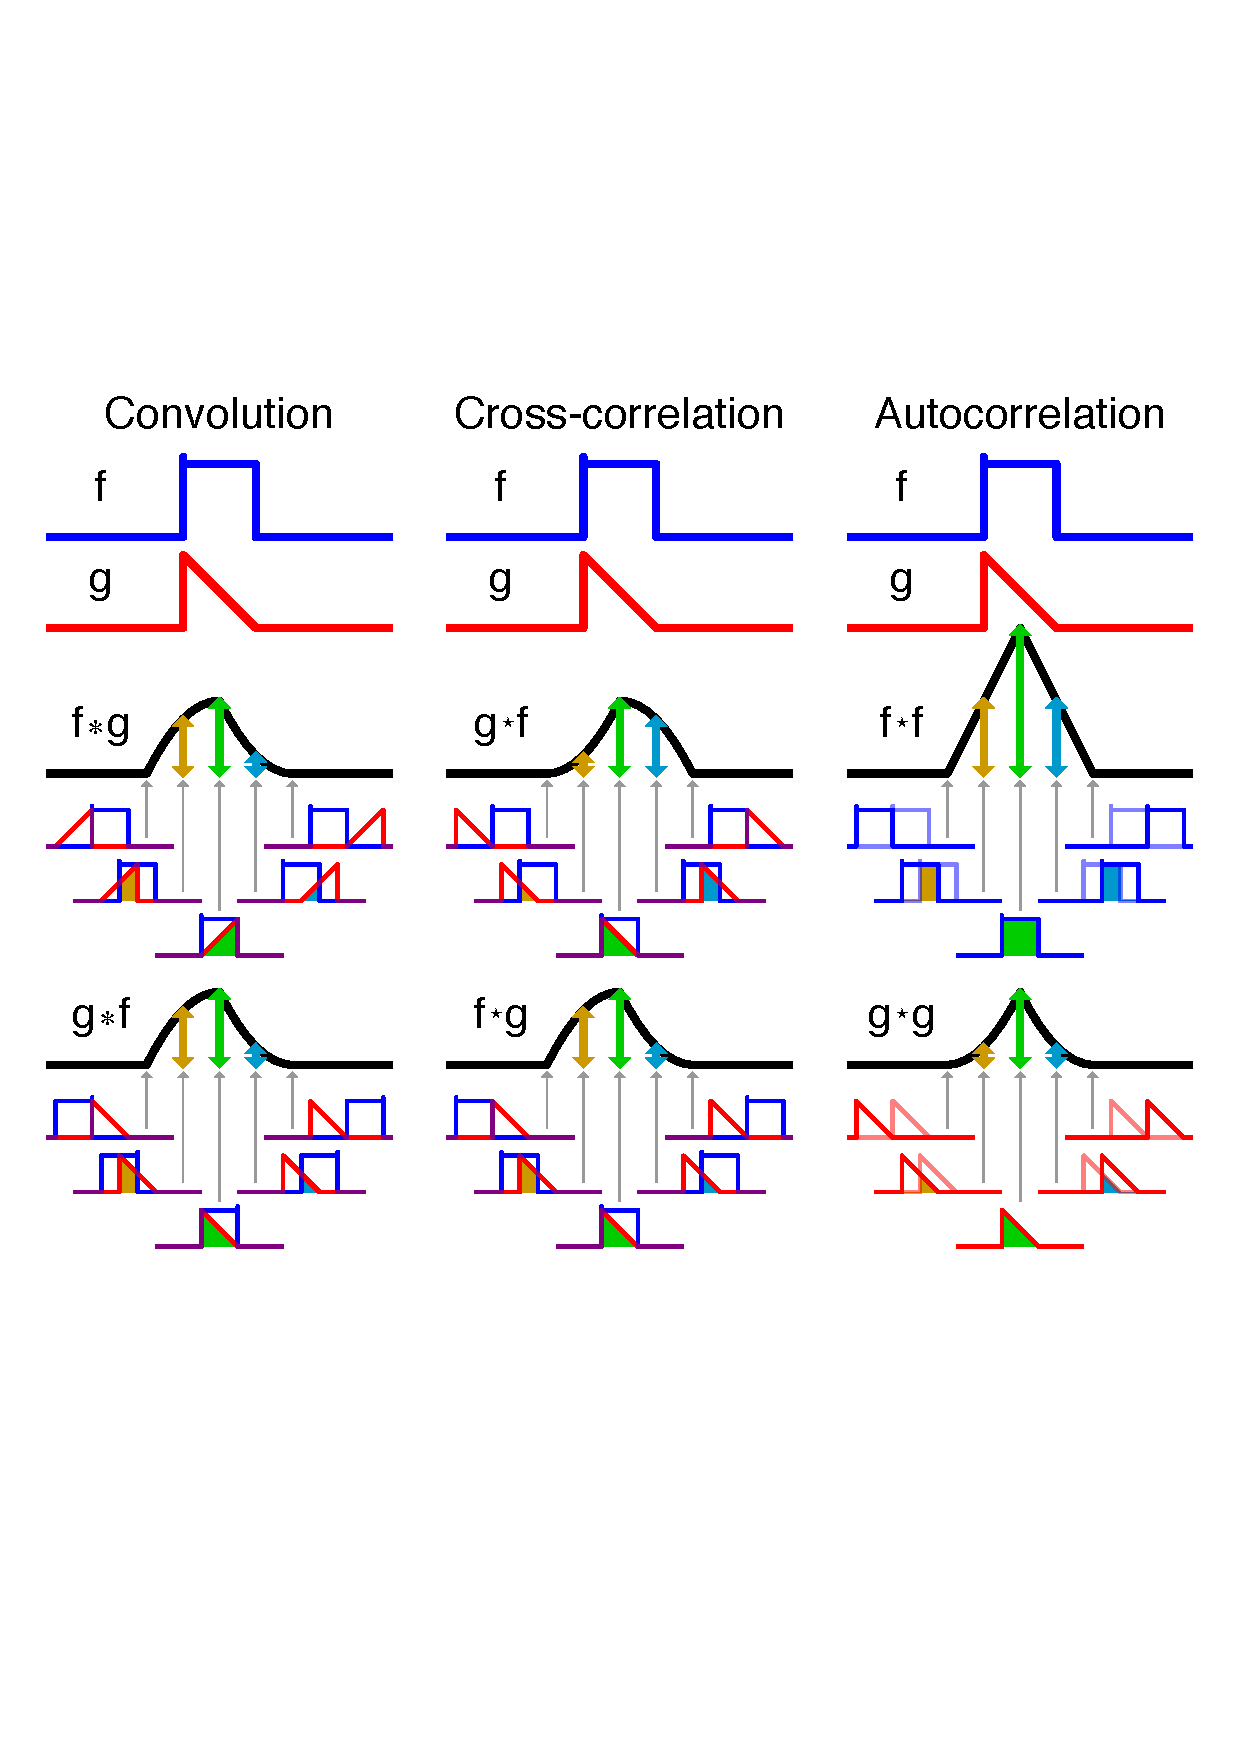
\includegraphics[width=0.6\textwidth]{figures/comparison_convolution_correlation}
  \caption{Graphical representation of a convolution and its comparison with correlation, image extracted from Wikipedia commons.}
  \label{fig:representation_convolution}
\end{figure}

A multidimensional convolution of infinite range the definition becomes \cite{multidimensionalConvolution}: 

\begin{figure}[!htp]
  \center
  \[f(t_1,t_2) \ast g(t_1,t_2) = \int_{t_1=-\infty}^{\infty}\int_{t_2=-\infty}^{\infty} f(\tau _1,\tau _2)g(t_1-\tau _1,t_2-\tau _2)d\tau _1 d\tau _2\]
  \caption{Multidimensional convolution for infinite ranges of $t_1,t_2 \in (-\infty, \infty)$}
  \label{fig:multidimension_convolution_infinite_range}
\end{figure}

In computer vision, images are transformed into two-dimensional functions, that can be represented as a matrix in which each value usually takes 0 or 1 values for black and white images or from 0 to 255 to gray-scale images. Most of the image transformations are based sliding window or function called ``kernel'', ``filter'' or ``feature detector'' \cite{cnnDennyBritz} represented in figure \ref{fig:convolution_filter}.

\begin{figure}[!htp]
  \center
  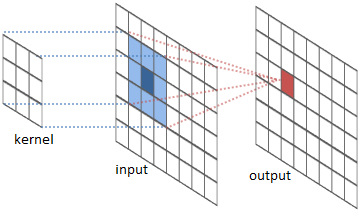
\includegraphics[width=0.6\textwidth]{figures/convolution_filter}
  \caption{Representation of a 2D image convolution transformation of filter size 3x3.}
  \label{fig:convolution_filter}
\end{figure}

\section{Convolutional Neural Networks}

\acrlong{cnn} are usually feed-forward type neural networks that concatenate multiple layers of convolutions with non linear activation functions as shown in figure \ref{fig:cnn_architecture}. The learning process of, for example, an image classification, consist on learning relevant values by detecting the edges of the raw pixel values in the input of the \acrshort{cnn}. Over the following layers with the extraction of high level features, until reaching to last fully connected layer in which, the objects are classified by using the previously extracted features. 

\begin{figure}[!htp]
  \center
  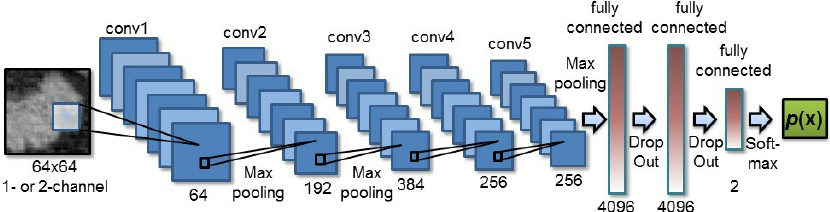
\includegraphics[width=0.96\textwidth]{figures/cnn_architecture}
  \caption{Example of a Convolutional Neural Network architecture \cite{kooi2017classifying}.}
  \label{fig:cnn_architecture}
\end{figure}

To apply the following architecture to \acrshort{nlp} related tasks, instead of a two dimension convolution array that represents the image, each row of the matrix represents a token, usually being this tokens numerical representations of words or characters as space vectors that are initialized with word2vec or GloVe algorithms. Then, as with images each convolution layer extract features that are used on the last layer to categorize the given document as shown in figure \ref{fig:cnn_npl}. 

There are multiple types of architectures that combine multiple pooling layers that reduce computation cost by sub-sampling the matrix on each filter. In addition, multiple channels of \acrshort{cnn} could be used to process different word embeddings in each channel or applying different filters per channel \cite{singhalborrow}, an idea origins from image processing to analyze each color.

\begin{figure}[htbp]
  \center
  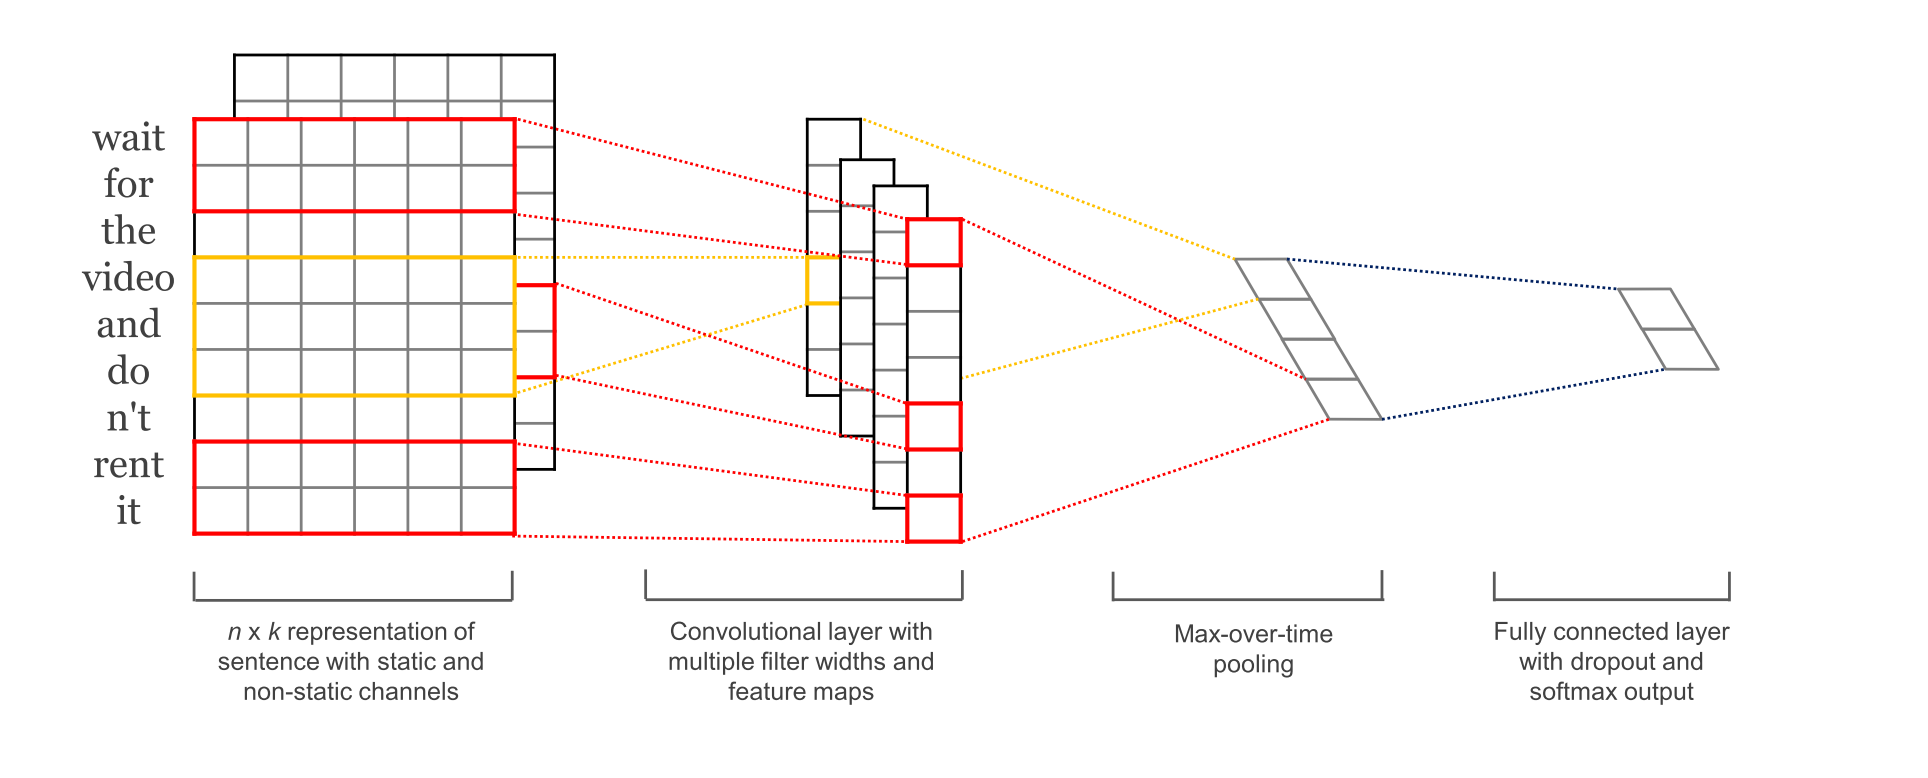
\includegraphics[width=0.7\textwidth]{figures/cnn_npl}
  \caption{Example of a Convolutional Neural Network architecture applied to NLP \cite{kim2014convolutional}.}
  \label{fig:cnn_npl}
\end{figure}
